\section{Deployment view}

In Abbildung~\ref{fig:deployment-diagram} ist eine Übersicht über das Deplyoment der Applikation und dazugehöriger
Services zu sehen.
\begin{figure}
    \centering
    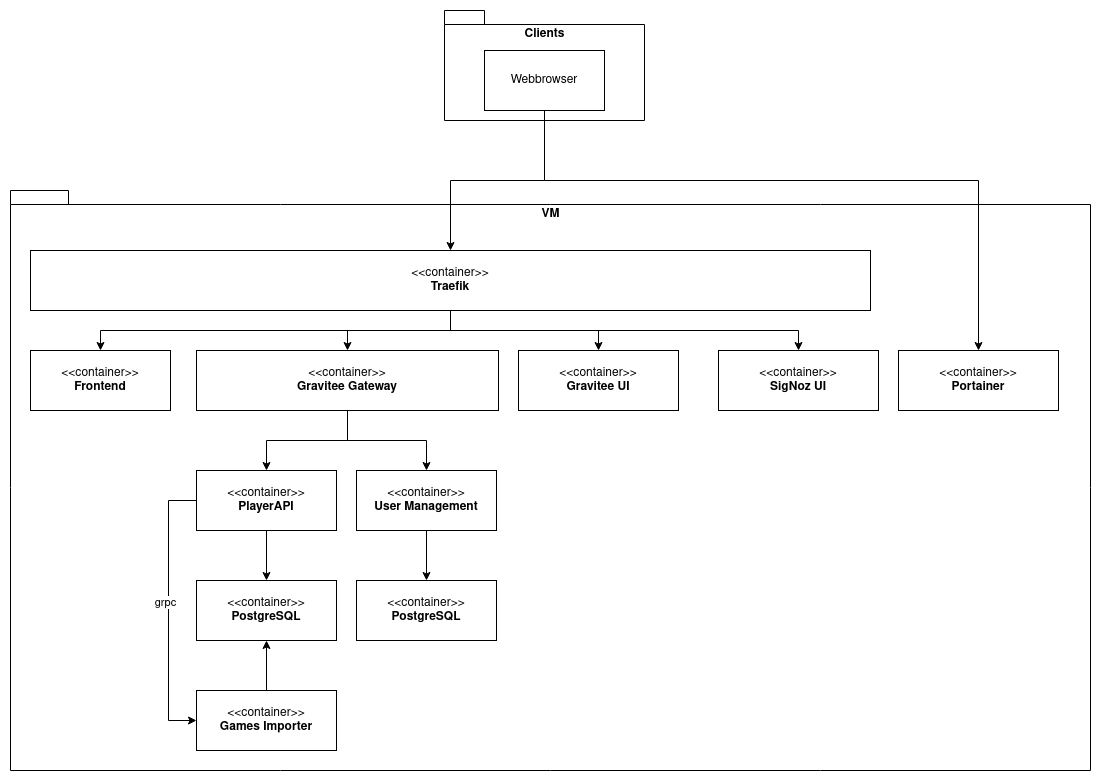
\includegraphics[width=\textwidth]{images/cdc-08-deployment-diagram.drawio}
    \caption{Deplyoment Diagramm}
    \label{fig:deployment-diagram}
\end{figure}

Die gesamte Applikation läuft innerhalb einer VM, wobei alles verdockert ist.
Das initiale Routing und bereitstellen von https Zertifikaten übernimmt ein Traefik Container.
So gibt es für jeden Teil eine eigene URL:
\begin{itemize}
    \item Frontend: lol-stats.de
    \item API (Gravitee Gateway): lol-stats.de/api
    \item Gravitee UI: api-ui.lol-stats.de
    \item SigNoz UI: tracing.lol-stats.de
\end{itemize}

Nur Portainer ist direkt über einen Port erreichbar, weil es keine gute Idee ist Traefik in Portainer einzurichten
und gleichzeitig Portainer nur über Traefik erreichbar zu machen.
Alle API Anfragen werden über das Gravitee Gateway geleitet.
Hierüber werden die internen API routen festgelegt.
Gravitee lässt sich über ein Webinterface in der Gravitee UI konfigurieren.
Die eingesammleten Traces lassen sich ebenfalls über ein Webinterface in der SigNoz UI anschauen.